\section{Resultados}

\subsection{Bases de datos disponibles}

\subsection{Validaci�n}

\subsection{Entendiendo las gr�ficas}


\subsection{Momentos vs Pseudo-inversa}
\subsection{Preprocesar o No Preprocesar}
\label{prepoceso}

Como se indic� en la secci�n \ref{sec:conceptos_preproceso}, antes del c�lculo de los features se suelen usar~$3$ filtros como preproceso. Estos filtros son: 1. suavizado, 2. resampling, y 3. resizing (no necesariamente en ese orden). En lo siguiente se desea examinar la posibilidad de eliminar estos pasos en pos de eficiencia.

% El algoritmo de c�lculo de momento puede ser implementado (como se vio en la sec) de manera tal que puedan ser calculados a medida que los datos se vayan introduciendo.

%Evitar utilizar estos filtros permitir�a el c�lculo de los momentos a medida que se van ingresando los datos, como se ha indicado en la secci�n \ref{sec:calculo_numerico_momentos}; lo cu�l permitir�a un aumento considerable de eficiencia en comparaci�n con el m�todo de la pseudo-inversa, el cual necesita esperar a que el usuario termine


\subsubsection{Evitando suavizado}
Recordar que los features son los coeficientes de polinomios, obtenidos por aproximaci�n de m�nimos cuadrados, lo cual genera una curva suave. El objetivo del suavizado (la eliminaci�n del ruido presente al principio y final de cada trazo) es alcanzado sin necesidad de realizar un filtrado. Entonces, no es necesario este paso.

\subsubsection{Evitando resampling}
Al cambiar la representaci�n de los trazos, de secuencia de puntos a curvas continuas, no hay necesidad de espaciarlos uniformemente o reducir/aumentar la cantidad de puntos en los trazos (tarea del filtro en cuesti�n). Si la velocidad en la que es escrito un s�mbolo afecta el reconocimiento, se puede optar por la reparametrizaci�n por longitud de arco, secci�n \ref{sec:arc-length}. Por lo tanto, tampoco es necesario el resampling.

\subsubsection{Evitando resizing}
Se ha demostrado que los features obtenidos son invariantes a escala, secci�n \ref{Invariante_escala}. Por lo que tambi�n es innecesario aplicar este filtro.

\subsubsection{Evitando traslaci�n}
Un filtro no mencionado es aplicar traslaci�n, que se ocupa de trasladar el trazo de manera tal que el m�nimo de cada eje sea $0$. Se ha expresado que los features no son invariantes a traslaci�n. Aqu� se muestra por experimentaci�n, que las traslaciones no provocan una p�rdida significativa en la precisi�n de reconocimiento. �sto permitir�a tomar dos caminos al implementar un sistema de reconocimiento: preprocesar o no hacerlo. Esta decisi�n de dise�o puede ser tomada para caso en que se requiera extrema eficiencia, como el caso de los dispositivos m�viles, evitando preprocesar a costa de perder precisi�n. Entonces, se tiene que evaluar en qu� escenario se desea utilizar el sistema de reconocimiento, y elegir el balance justo entre eficiencia y precisi�n seg�n sea el caso. Una comparaci�n sobre la precisi�n de reconocimiento puede verse en~\ref{fig:prep_vs_no_prep}.
\vspace*{-0.3cm}
\begin{figure}[!htbp]
  \centering
  \advance\leftskip-2.8cm
  \advance\rightskip-2.8cm
  \subfloat[Sin prepoceso]{\label{fig:prep}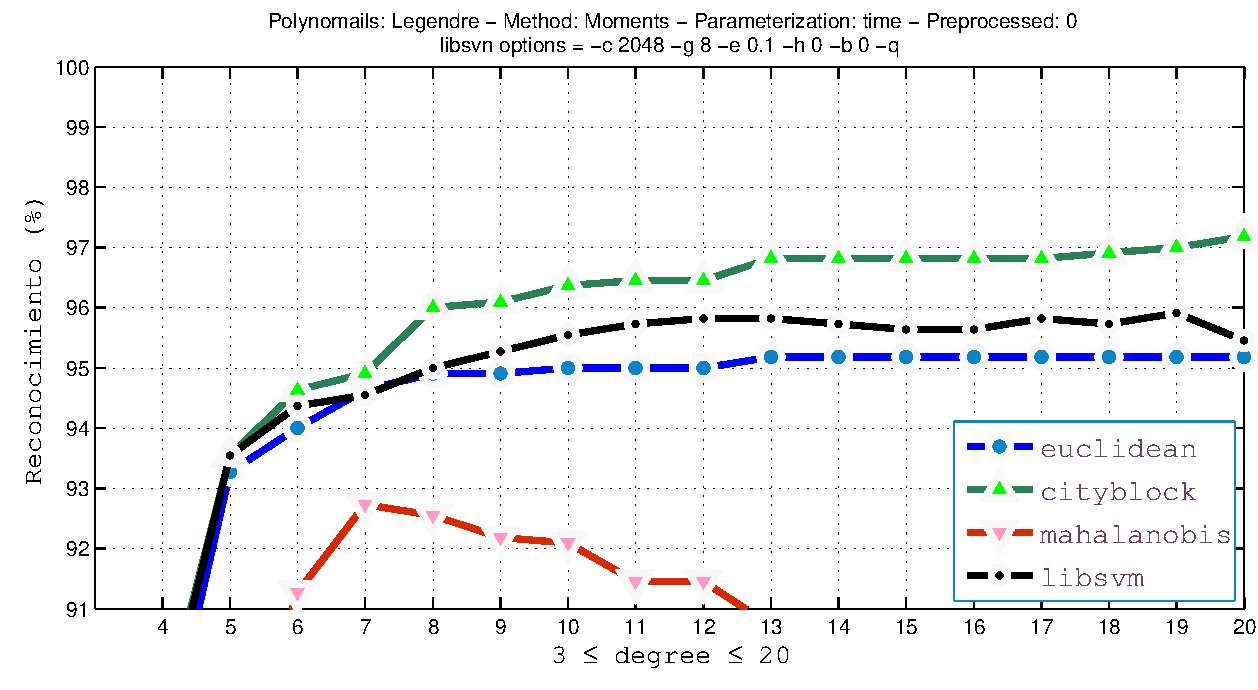
\includegraphics[scale=0.46,keepaspectratio=true]{imagen/plot/moments_L_preproceso_0.pdf}}
  \subfloat[Con prepoceso]{\label{fig:no_prep}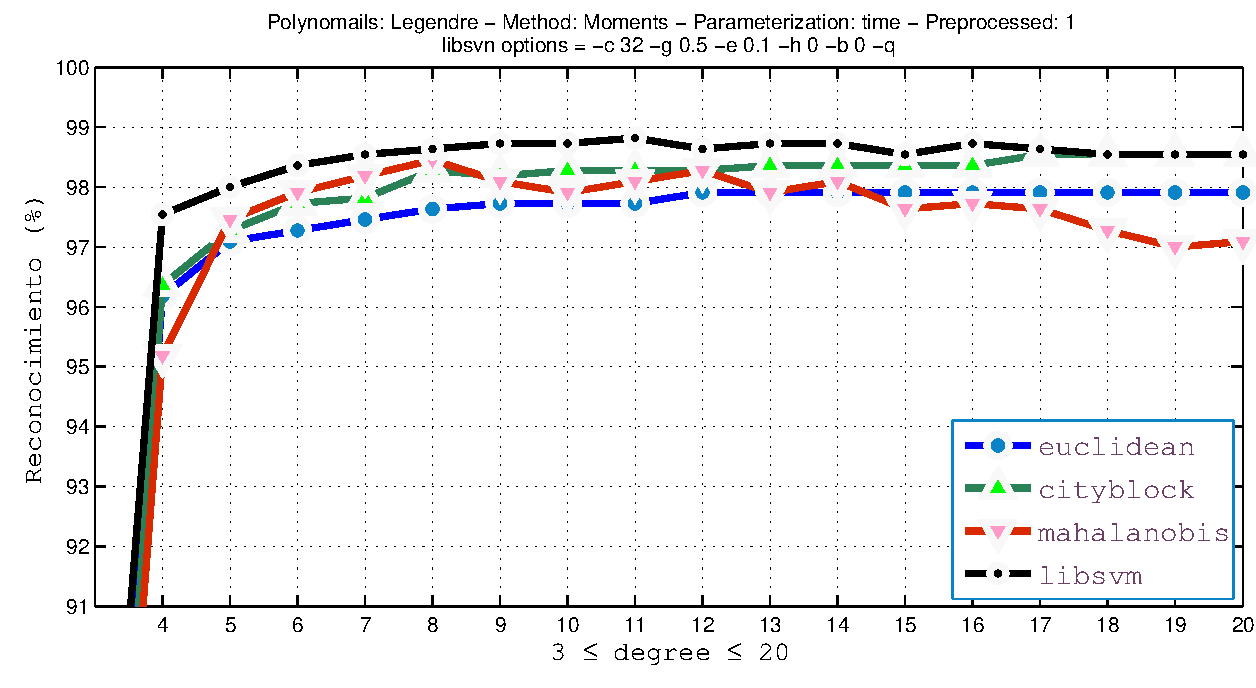
\includegraphics[scale=0.46,keepaspectratio=true]{imagen/plot/moments_L_preproceso_1.pdf}}
  \caption{Momentos con polinomios de Legendre}
  \label{fig:prep_vs_no_prep}
\end{figure}


% \begin{figure}[h!]
%  \centering
%  \advance\leftskip-2.8cm
%  \advance\rightskip-2.8cm
%  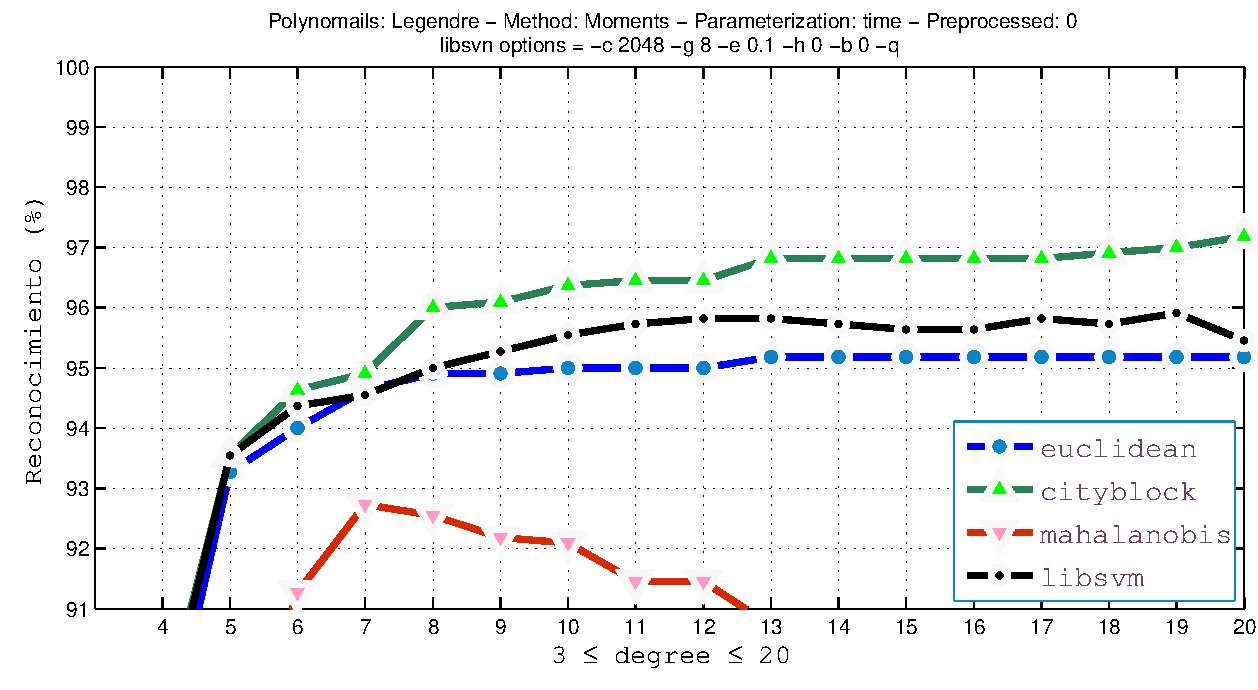
\includegraphics[scale=0.46,keepaspectratio=true]{imagen/plot/moments_L_preproceso_0.pdf}
% \hspace*{-0.4cm}
% 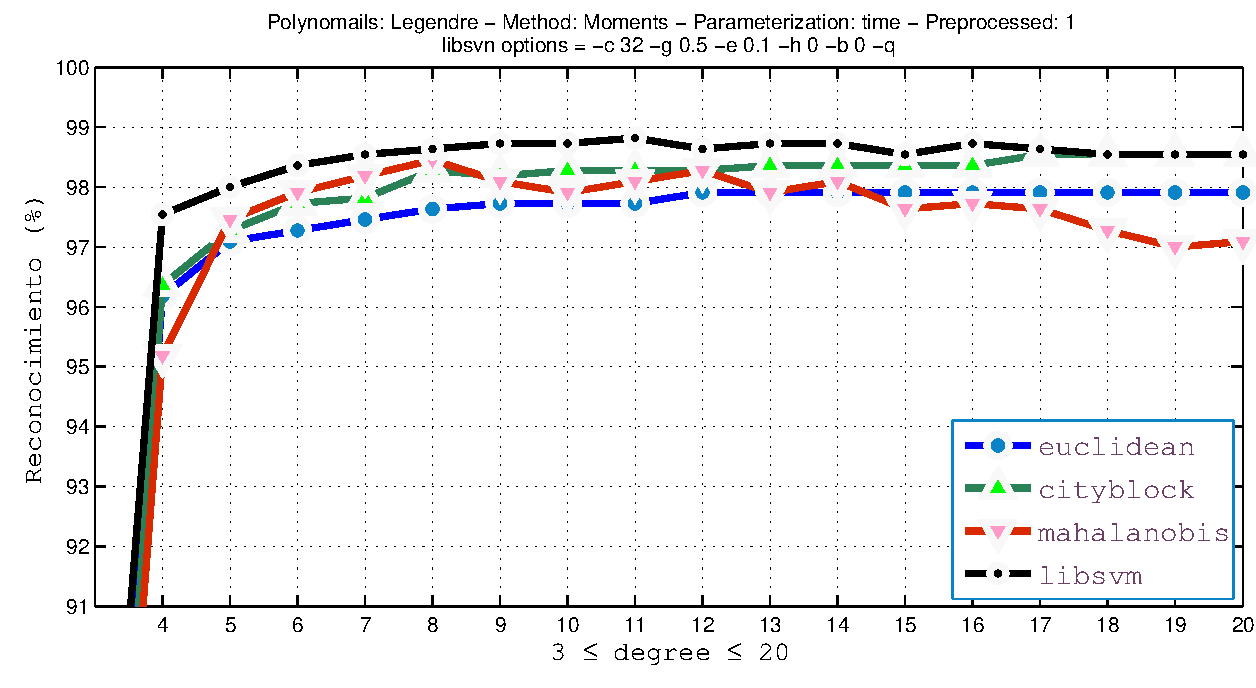
\includegraphics[scale=0.46,keepaspectratio=true]{imagen/plot/moments_L_preproceso_1.pdf}
%  \caption{Sin preproceso (izq.), y con preproceso (der.). M�todo: Momentos con polinomios de Legendre}
%  \label{fig:prep_vs_no_prep}
% \end{figure}



%  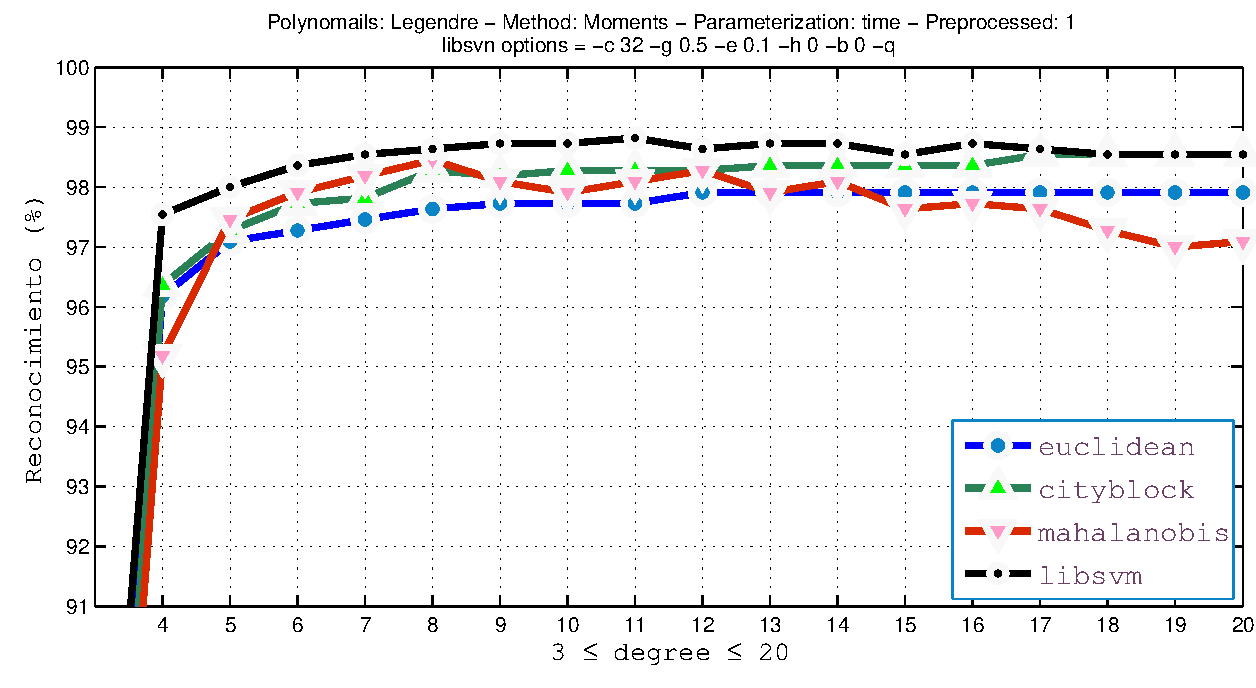
\includegraphics[scale=0.458,keepaspectratio=true]{imagen/plot/moments_L_preproceso_1.pdf}
%  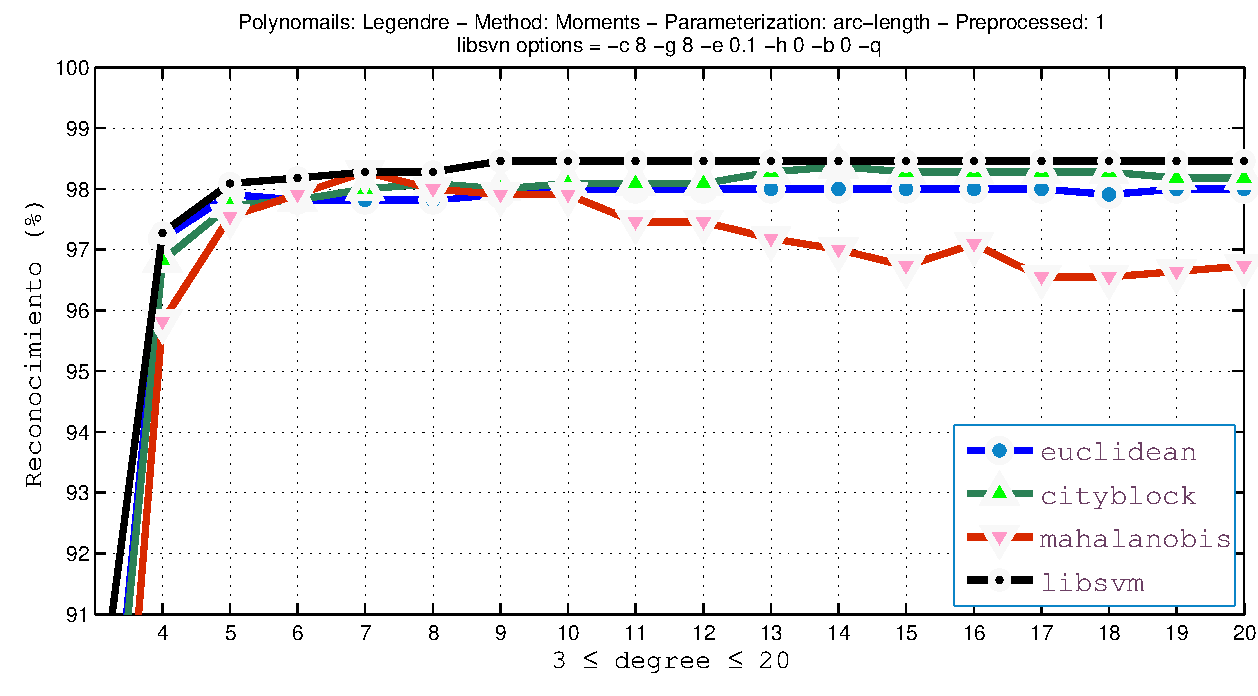
\includegraphics[scale=0.46,keepaspectratio=true]{imagen/plot/moments_L_arc_preproceso_1.pdf}


\subsection{Parametrizaci�n por tiempo vs Parametrizaci�n por longitud de arco}
\subsection{Representaci�n a elegir: Legendre, Chebyshev o Legendre-Sobolev}

\subsection{Momentos como features}

\subsection{Mejor performance}
\subsection{Mejor precisi�n}
